
%%%%%%%%
\Intercalaire{Introduction au calcul statistique avec PROCOR/URANIE}
\section{Introduction au calcul statistique avec PROCOR/URANIE}
\Titre{Introduction au calcul statistique avec PROCOR/URANIE}
\begin{frame}[fragile]
Pourquoi des calculs statistiques ?
\begin{itemize}
\item Gérer la méconnaissance de paramètres ou de données d'entrée au système à résoudre.
\item Participer à l'amélioration de la connaissance de la phénoménologie (cf. transparent "La démarche phénoménologique dans PROCOR").
\end{itemize}

3 catégories d’incertitudes :

\begin{itemize}
\item Aléatoires (e.g. précision du système de mesure, fluctuation de l’environnement…) et
incompressibles
\begin{itemize}
\item densité de probabilité (pdf)
\end{itemize}
\item Épistémiques (manque de connaissance)
\begin{itemize}
\item \textit{a priori} pas de pdf
\item Expertise : plage de variation
\item Une pdf peut-être supposée (degré de croyance)
\end{itemize}
\item Mixtes (aléatoire et épistémiques)
\end{itemize}



\end{frame}



\Titre{Introduction au calcul statistique avec PROCOR/URANIE}
\begin{frame}[fragile]

Approche probabiliste des incertitudes dans la simulation :
\begin{itemize}
\item Grandeurs incertaines \(\rightarrow\) Variables aléatoires
\begin{itemize}
\item Incertitudes = densité de probabilité (pdf) de la variable aléatoire
\end{itemize}
\end{itemize}

Processus typique des études statistiques :


\begin{figure}
\centering 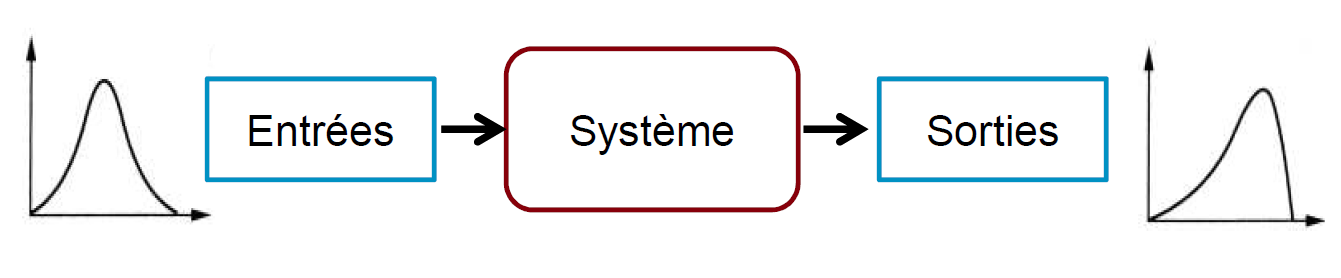
\includegraphics[width=0.75\textwidth]{Figures/Stat_1.png} 
\end{figure}


\end{frame}


\Titre{Introduction au calcul statistique avec PROCOR/URANIE}
\begin{frame}[fragile]
Qu'entend-on par "études statistiques" ?
\begin{itemize}
\item Etudes paramétriques
\begin{itemize}
\item Définition d’une plage de variation d’Entrées
\(\rightarrow\) plage de variation des Sorties
(palliatif au manque de connaissance des Entrées)
\end{itemize}
\item Analyse de sensibilité (incertitudes avec pdf )

\begin{itemize}
\item A partir des incertitudes des Entrées
\(\rightarrow\) quantifier la sensibilité du système à chaque Entrée
(classement des Entrées par degré d’influence)
\end{itemize}

\item Propagation d’incertitudes
\begin{itemize}
\item A partir des incertitudes (exhaustives et précises) des Entrées
\(\rightarrow\) Incertitudes des Sorties
(précision du calcul)
\end{itemize}

\end{itemize}

\end{frame}




\Titre{Introduction au calcul statistique avec PROCOR/URANIE}
\begin{frame}[fragile]
Sources d'incertitudes pour les Accidents Graves
\begin{figure}
\centering 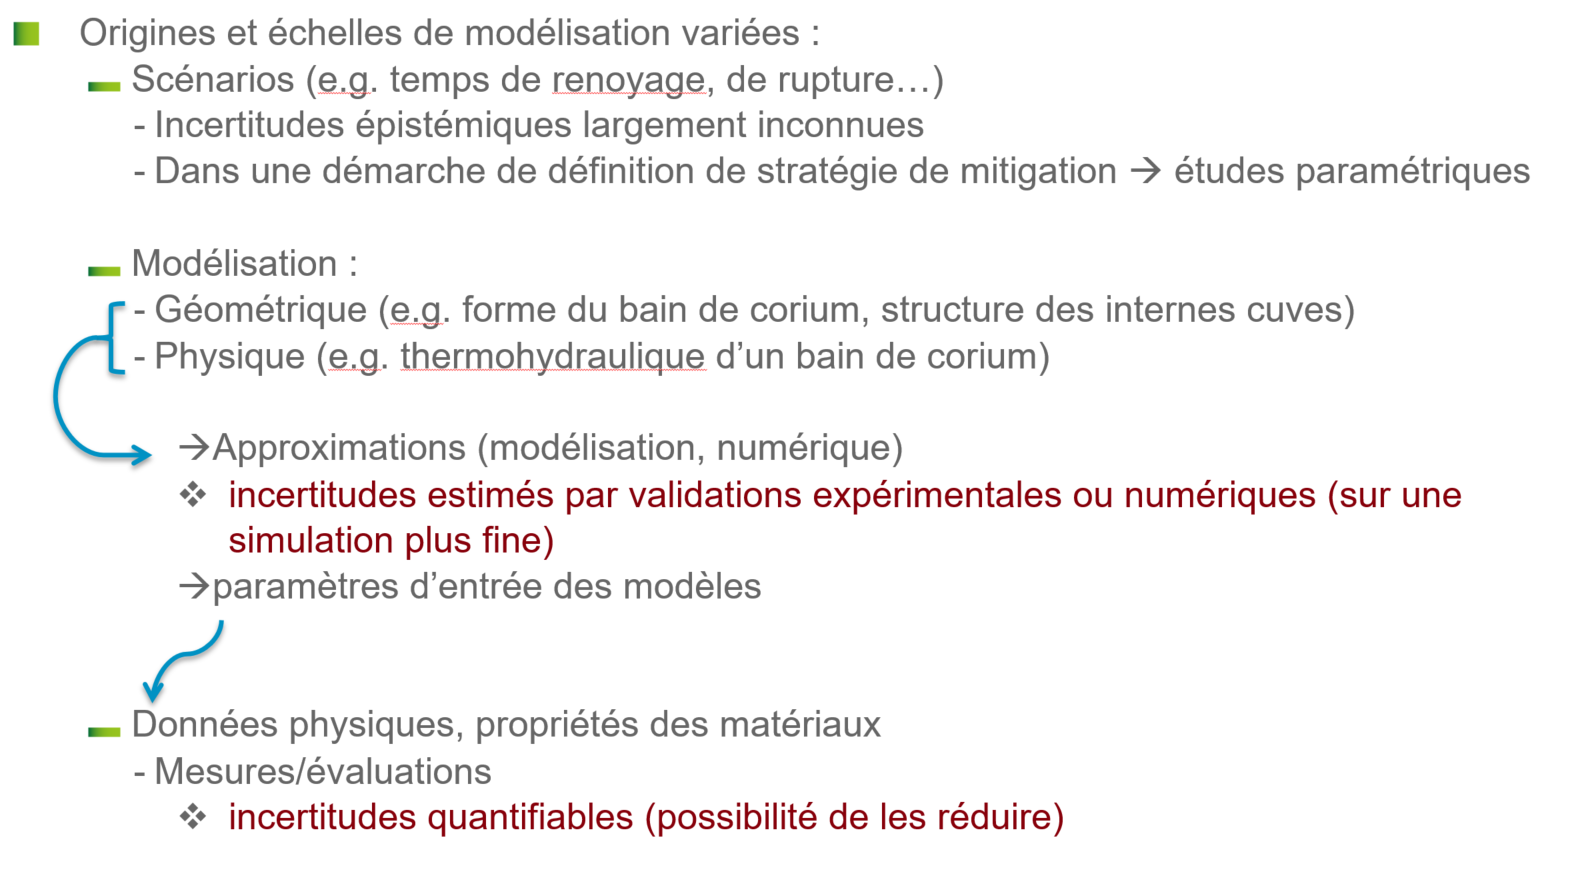
\includegraphics[width=0.95\textwidth]{Figures/Stat_OriginesIncert.png} 
\end{figure}


\end{frame}


\Titre{Introduction au calcul statistique avec PROCOR/URANIE}
\begin{frame}[fragile]
En pratique, un \emph{outil spécifique pour PROCOR} (\textit{statistics}) a été construit sur la base de la plateforme URANIE.\\
\emph{URANIE} est la plateforme du CEA pour la propagation d'incertitudes, elle-même basée sur l'outil \emph{ROOT} du CERN.
Cela permet une utilisation facilité des fonctionnalités d'URANIE. Les grandes étapes sont: 
\begin{itemize}
\item définition des paramètres d'entrée à probabiliser \\
dans un fichier \textit{template} du même type que \texttt{ap1000\_benchmark\_parameter\_input\_file.txt} , en remplaçant la valeur du paramètre par \textit{xxx}

\item définition des loi statistiques suivies par les pdf de ces paramètres et du nombre de calculs à réaliser\\
dans un fichier spécifique \texttt{input.uranie}

\item définition des paramètres de sortie qui seront observés \\
dans un fichier \texttt{output.uranie} permettant de renommer les sorties avec des alias et de leur donner une valeur par défaut.

\end{itemize}

\end{frame}


\Titre{Introduction au calcul statistique avec PROCOR/URANIE}
\begin{frame}[fragile]


Processus du calcul statistique : 
\begin{itemize}
    \item échantillonnage (tirage aléatoire) des valeurs des paramètres d'entrée compte tenu de leur loi de pdf et du nombre de calcul à effectuer
    \item création des fichiers d'entrée \texttt{ap1000\_benchmark\_parameter\_input\_file.txt} pour chaque calcul
    \item lancement des calculs
    \item récupération des valeurs des sorties observées dans un tableau comprenant les valeurs des entrées et des sorties
\end{itemize}



\end{frame}


\Titre{Introduction au calcul statistique avec PROCOR/URANIE}
\begin{frame}[fragile]
L'outil \textit{statistics} calcule deux grandeurs :
\begin{itemize}
    \item la probabilité d'un évènement (variable aléatoire \textit{X}, entre 0 et 1)
\end{itemize}
\begin{figure}
\centering 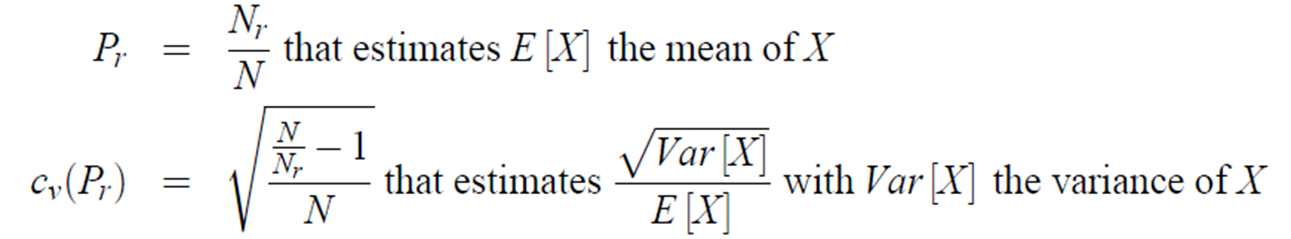
\includegraphics[width=0.95\textwidth]{Figures/Stat_EventProba.png} 
\end{figure}

\begin{itemize}
    \item le ratio de corrélation d'un paramètre \textit{P} étant donné un évènement \textit{X}
\end{itemize}
\begin{figure}
\centering 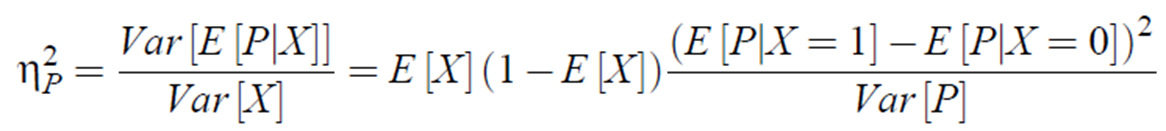
\includegraphics[width=0.95\textwidth]{Figures/Stat_CorrelationRatio.png} 
\end{figure}



\end{frame}


\Titre{Introduction au calcul statistique avec PROCOR/URANIE}
\begin{frame}[fragile]
Le post-traitement avec ROOT est à la charge de l'utilisateur. Cf. page du wiki PROCOR pour l'utilisation de ROOT pour PROCOR (fournie séparément).


\begin{itemize}
    \item Mise en pratique sur le cas n°3. Pour des raisons de temps de calculs, les calculs ont déjà été réalisés avec un choix des paramètres d'entrée probabilisés : 
    
    \begin{itemize}
        \item A définir
    \end{itemize}
\end{itemize}

    \item Objectif : identifier les paramètres d'entrée influents et choisir la meilleur représentation pour illustrer ce choix.



\end{frame}
